\documentclass[text05.tex]{subfiles}
\begin{document}
\subsubsection{\ruby{距離}{きょ|り}センサー}\label{distance}
\begin{table}[H]
	\begin{widerrows}
		\begin{tabular}{|p{\colF}|p{\colG}|} \hline
		\ruby{名称}{めい|しょう} & \ruby{距離}{きょ|り}センサー（きょりせんさー）\\ \hline
		\ruby{接続箇所}{せつ|ぞく|か|しょ} & アナログコネクタ (3pin)\\ \hline
		\ruby{機能概要}{き|のう|がい|よう} & センサーから\ruby{障害物}{しょう|がい|ぶつ}までの\ruby{距離}{きょ|り}を\ruby{計測}{けい|そく}\\ \hline
		\end{tabular}
  \end{widerrows}	
\end{table}

\begin{table}[H]
	\begin{widerrows}
		\begin{tabular}{|p{\colF}|p{\colG}|}	\hline
		サンプルコードの場所 & 05/anain.hsp\\ \hline
		raspiへの入力 & \ruby{距離}{きょ|り}をあらわす0から1023の\ruby{値}{あたい}。\ruby{測定可能}{そく|てい|か|のう}な\ruby{距離}{きょ|り}は10cmから80cm。\\ \hline
		raspiへの入力方法 & val = \adcget(ピン番号, チャンネル番号)\\ \hline
		raspiからの出力 & なし\\ \hline
		raspiからの出力方法 & なし\\ \hline
		\end{tabular}
  \end{widerrows}	
\end{table}

\begin{table}[H]
	\begin{widerrows}
		\begin{tabular}{|p{\colF}|p{\colG}|} \hline
		使い道 & \ruby{距離}{きょ|り}\ruby{計測}{けい|そく}、\ruby{障害物}{しょう|がい|ぶつ}センサーとして。\\ \hline
		\ruby{注意事項}{ちゅう|い|じ|こう} & レンズを\ruby{覗}{のぞ}き\ruby{込}{こ}むと目に\ruby{影響}{えい|きょう}を\ruby{及}{およ}ぼすことがあるため\ruby{覗}{のぞ}き\ruby{込}{こ}まないこと。\\ \hline
		\ruby{補足}{ほ|そく} & センサーからの入力はセンチメートルではなく、ADCが読み取った0から1023までの\ruby{値}{あたい}です。ここでは、使用している\ruby{距離}{きょ|り}センサーとADCに合わせて実験的に求めた\ruby{近似式}{きん|じ|しき}を使い、\ruby{入力値}{にゅう|りょく|ち}を\ruby{距離}{きょ|り}（センチメートル）に\ruby{換算}{かん|さん}します。数式\ref{eq:distance}の$x$にセンサーからの\ruby{値}{あたい}を代入すると、10cmから80cm\ruby{程度}{てい|ど}の\ruby{範囲}{はん|い}でおよその\ruby{距離}{きょ|り}を求めることができます。この式は、\ruby{異}{こと}なるセンサーやADCにはそのまま使えません。
		\begin{equation}
		\frac{3952640}{875 \times x + 22272}
		\label{eq:distance}
		\end{equation}
	この\ruby{距離}{きょ|り}センサーは、赤外線を出す\ruby{光源}{こう|げん}と、\ruby{反射}{はん|しゃ}して\ruby{戻}{もど}ってきた光を受ける受光器でできています。物体までの\ruby{距離}{きょ|り}が変わると、受光器に光が\ruby{届}{とど}く位置も変わります。\ruby{光源}{こう|げん}と受光器の位置は固定されているため、この位置の変化を利用して、\ruby{三角測量}{さん|かく|そく|りょう}の原理で物体までの\ruby{距離}{きょ|り}を求めます。\\ \hline
		\end{tabular}
  \end{widerrows}	
\end{table}

\begin{figure}[H]
	\begin{widerrows}
		\begin{tabular}{|p{\colH}|p{\colI}|p{\colH}|p{\colI}|} \hline
		外観 & 
		\begin{minipage}[t]{\linewidth}
			\smallskip
				\centering
				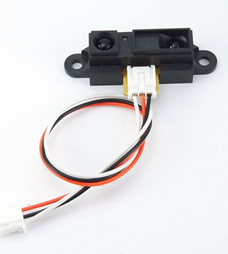
\includegraphics[width=0.5\linewidth]{../../asset/image/text05-img031.png}
				\caption{\ruby{距離}{きょ|り}センサー}
				\smallskip
			\end{minipage} &
			回路記号 & 回路記号はありません。\\ \hline
		\end{tabular}
  \end{widerrows}	
\end{figure}
\end{document}
